\documentclass[12pt]{report}
\usepackage[utf8]{inputenc}
%\usepackage[14pt]{extsizes}
\usepackage{listings}
\usepackage{indentfirst}
\usepackage{geometry}
\usepackage{textcomp}
\usepackage{amssymb}
\usepackage{amsmath}
\usepackage{amsthm} 
\usepackage{caption}
\usepackage{misccorr}
\usepackage[noadjust]{cite}
\usepackage{cmap} 
\usepackage[T2A]{fontenc}
\usepackage[english, russian]{babel}
\usepackage{graphics}
\usepackage{graphicx}
\usepackage{textcomp}
\usepackage{verbatim}
\usepackage{makeidx}
\usepackage{float}
\usepackage{bm}
\usepackage{esint}
\usepackage{mathtools}
\usepackage{graphicx}
\usepackage{listings}
% Для листинга кода:
\lstset{ %
language=python,                 % выбор языка для подсветки (здесь это С)
basicstyle=\small\sffamily, % размер и начертание шрифта для подсветки кода
numbers=left,               % где поставить нумерацию строк (слева\справа)
numberstyle=\tiny,           % размер шрифта для номеров строк
stepnumber=1,                   % размер шага между двумя номерами строк
numbersep=5pt,                % как далеко отстоят номера строк от подсвечиваемого кода
showspaces=false,            % показывать или нет пробелы специальными отступами
showstringspaces=false,      % показывать или нет пробелы в строках
showtabs=false,             % показывать или нет табуляцию в строках
frame=single,              % рисовать рамку вокруг кода
tabsize=2,                 % размер табуляции по умолчанию равен 2 пробелам
captionpos=t,              % позиция заголовка вверху [t] или внизу [b] 
breaklines=true,           % автоматически переносить строки (да\нет)
breakatwhitespace=false, % переносить строки только если есть пробел
escapeinside={\#*}{*)}   % если нужно добавить комментарии в коде
}

% Для измененных титулов глав:
\usepackage{titlesec, blindtext, color} % подключаем нужные пакеты
\definecolor{gray75}{gray}{0.75} % определяем цвет
\newcommand{\hsp}{\hspace{20pt}} % длина линии в 20pt
% titleformat определяет стиль
\titleformat{\chapter}[hang]{\Huge\bfseries}{\thechapter\hsp\textcolor{gray75}{|}\hsp}{0pt}{\Huge\bfseries}

\makeatletter
\def\@biblabel#1{#1. }
\makeatother

\usepackage{hyperref}

\newcommand{\specchapter}[1]{\chapter*{#1}\addcontentsline{toc}{chapter}{#1}}
\newcommand{\specsection}[1]{\section*{#1}\addcontentsline{toc}{section}{#1}}
\newcommand{\specsubsection}[1]{\subsection*{#1}\addcontentsline{toc}{subsection}{#1}}

% геометрия
\geometry{pdftex, left = 2cm, right = 2cm, top = 2.5cm, bottom = 2.5cm}

\titlespacing{\chapter}{0pt}{-30pt}{20pt}

\setcounter{tocdepth}{4} % фикс переноса 
\righthyphenmin = 2
\tolerance = 2048

\begin{document}
%\def\chaptername{} % убирает "Глава"
\thispagestyle{empty}
\renewcommand\bibname{Список литературы}

\vspace{\baselineskip}
\noindent \begin{minipage}{0.15\textwidth}
	
\includegraphics[width=\linewidth]{bmstu}
\end{minipage}
\noindent\begin{minipage}{0.9\textwidth}
	\centering
	\textbf{Министерство науки и высшего образования Российской Федерации}\\
	\textbf{Федеральное государственное бюджетное образовательное учреждение высшего образования}\\
	\textbf{«Московский государственный технический университет имени Н.Э.~Баумана}\\
	\textbf{(национальный исследовательский университет)»}\\
	\textbf{(МГТУ им. Н.Э.~Баумана)}
\end{minipage}

\noindent\rule{18cm}{3pt}
\newline\newline
\noindent ФАКУЛЬТЕТ $\underline{\text{«Информатика и системы управления»}}$ \newline\newline
\noindent КАФЕДРА $\underline{\text{«Программное обеспечение ЭВМ и информационные технологии»}}$\newline\newline\newline\newline\newline\newline\newline


\begin{center}
\Large\textbf{Лабораторная работа № 1}
\end{center}
\vspace{\baselineskip}
\noindent\textbf{Дисциплина} $\underline{\text{Анализ алгоритмов~~~~~~~~~~~~~~~~~~~~~~~~~~~~~~~}}$\newline\newline
\noindent\textbf{Тема} $\underline{\text{Расстояния Левенштейна и Дамерау-Левенштейна}}$\newline\newline
\noindent\textbf{Студент} $\underline{\text{Куликов Д. А.~~~~~~~~~~~~~~~~~~~~~~~~~~~~~~~~~~~~~~~~~~~~~}}$\newline\newline
\noindent\textbf{Группа} $\underline{\text{ИУ7-52Б~~~~~~~~~~~~~~~~~~~~~~~~~~~~~~~~~~~~~~~~~~~~~~~~~~~~~~}}$\newline\newline
\noindent\textbf{Оценка (баллы)} $\underline{\text{~~~~~~~~~~~~~~~~~~~~~~~~~~~~~~~~~~~~~~~~~~~~~~~~~~~~~}}$\newline\newline
\noindent\textbf{Преподаватель} $\underline{\text{Волкова Л. Л.~~~~~~~~~~~~~~~~~~~~~~~~~~~~~~~~~~~}}$\newline

\begin{center}
	\vfill
	Москва~---~\the\year
	~г.
\end{center}
\clearpage

\tableofcontents

\newpage
\chapter*{Введение}
\addcontentsline{toc}{chapter}{Введение}
\textbf{Расстояние Левенштейна} — метрика, измеряющая разность между двумя последовательностями символов. Она определяется как минимальное количество односимвольных операций (а именно вставки, удаления, замены), необходимых для превращения одной последовательности символов в другую. В общем случае, операциям, используемым в этом преобразовании, можно назначить разные цены \cite{levbook}.\vspace{\baselineskip}

Расстояние Левенштейна широко используется в теории информации и компьютерной лингвистике. Примеры использования:

\begin{itemize}
	\item исправление ошибок в слове;
	\item в биоинформатике для сравнения генов, хромосом и белков;
	\item сравнение текстовых файлов утилитой diff и ей подобными.
\end{itemize}

\textbf{Цель работы:} изучение и применение на практике алгоритмов нахождения расстояния Левенштейна и Дамерау-Левенштейна, а также получение практических навыков реализации этих алгоритмов и сравнении их между собой.\vspace{\baselineskip} 

\textbf{Задачи работы:}
\begin{enumerate}
  	\item изучение алгоритмов Левенштейна и Дамерау-Левенштейна нахождения расстояния между строками;
	\item получение практических навыков реализации указанных алгоритмов: двух алгоритмов в матричной версии и одного из алгоритмов в рекурсивной версии; 
	\item сравнительный анализ линейной и рекурсивной реализаций выбранного алгоритма определения расстояния между строками по затрачиваемым ресурсам (времени и памяти); 
	\item экспериментальное подтверждение различий во временной эффективности рекурсивной и
нерекурсивной реализаций выбранного алгоритма определения расстояния между строками при
помощи разработанного программного обеспечения на материале замеров процессорного времени
выполнения реализации на варьирующихся длинах строк; 
	\item описание и обоснование полученных результатов в отчете о выполненной лабораторной
работе, выполненного как расчётно-пояснительная записка к работе. 
\end{enumerate}


\chapter{Аналитическая часть}
Задача по нахождению расстояния Левенштейна заключается в поиске минимального количества операций вставки/удаления/замены для превращения одной строки в другую.\vspace{\baselineskip}

При нахождении расстояния Дамерау-Левенштейна добавляется операция транспозиции (перестановки соседних символов).\vspace{\baselineskip}  
 
\textbf{Операции обозначаются следующим образом:} 
\begin{enumerate}
  	\item D (англ. delete) — удалить;
	\item I (англ. insert) — вставить;
	\item R (англ. replace) — заменить;
	\item M (англ. match) — совпадение;
	\item T (англ. transpose) — перестановка.
\end{enumerate}
Операция М имеет штраф 0, другие операции — штраф 1.

\section{Описание расстояний}
Пусть $S_{1}$ и $S_{2}$ — две строки (длиной M и N соответственно) над некоторым алфавитом, тогда расстояние Левенштейна можно подсчитать по следующей рекуррентной формуле:

\begin{displaymath}
D(i,j) = \left\{ \begin{array}{ll}
 0, & \textrm{$i = 0, j = 0$}\\
 i, & \textrm{$j = 0, i > 0$}\\
 j, & \textrm{$i = 0, j > 0$}\\
min(\\
D(i,j-1)+1,\\
D(i-1, j) +1, &\textrm{$j>0, i>0$}\\
D(i-1, j-1) + m(S_{1}[i], S_{2}[j])\\
),
  \end{array} \right.
\end{displaymath}

где $m(a,b)$ равна нулю, если $a=b$ и единице в противном случае; $min\{\,a,b,c\}$ возвращает наименьший из аргументов.

Расстояние Дамерау-Левенштейна вычисляется по следующей рекуррентной формуле:
\begin{displaymath}
D(i,j) = \left\{ \begin{array}{ll}
 0, & \textrm{$i = 0, j = 0$}\\
 i, & \textrm{$j = 0, i > 0$}\\
 j, & \textrm{$i = 0, j > 0$}\\
min(&\textrm{если $i,j>1$ and $a_{i} = b_{j-1},a_{i-1}=b_{j} $}\\
D(i,j-1)+1,\\
D(i-1, j) +1,\\
D(i-1, j-1) + m(S_{1}[i], S_{2}[j])\\
D(i-2, j-2) + 1,\\
)\\
min(&\textrm{иначе}\\
D(i,j-1)+1,\\
D(i-1, j) +1,\\
D(i-1, j-1) + m(S_{1}[i], S_{2}[j])\\
)
  \end{array} \right.
\end{displaymath}



\chapter{Конструкторская часть}
В этом разделе содержатся cхемы алгоритмов нахождения расстояний Левенштейна и Дамерау-Левенштейна и сравнительный анализ матричной и рекурсивной реализаций.

\section{Схемы алгоритмов}
На рис. 2.1-2.4 приведены схемы следующих алгоритмов:
\begin{enumerate}
	\item матричный алгоритм нахождения расстояния Левенштейна;
	\item рекурсивный алгоритм нахождения расстояния Левенштейна;
	\item рекурсивный алгоритм нахождения расстояния Левенштейна с заполнением 
	матрицы;
	\item матричный алгоритм нахождения расстояния Дамерау-Левенштейна.
\end{enumerate}
\newpage
\begin{figure}[h]
	\center{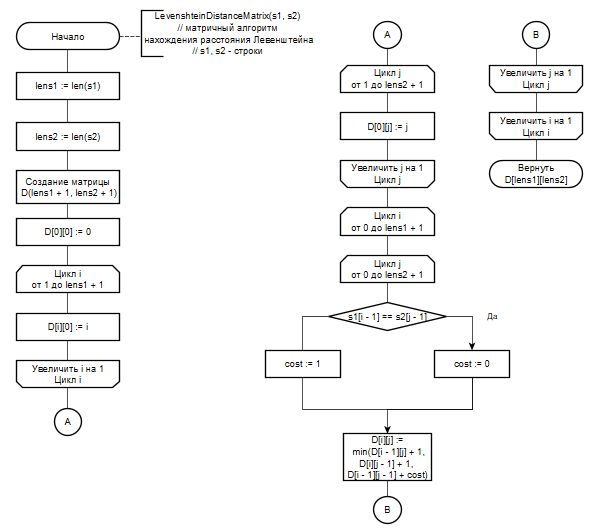
\includegraphics[scale=1]{LevMatr}}
	\caption{Матричный алгоритм нахождения расстояния Левенштейна}
	\label{figure:image}
\end{figure}
\newpage
\begin{figure}[h]
	\center{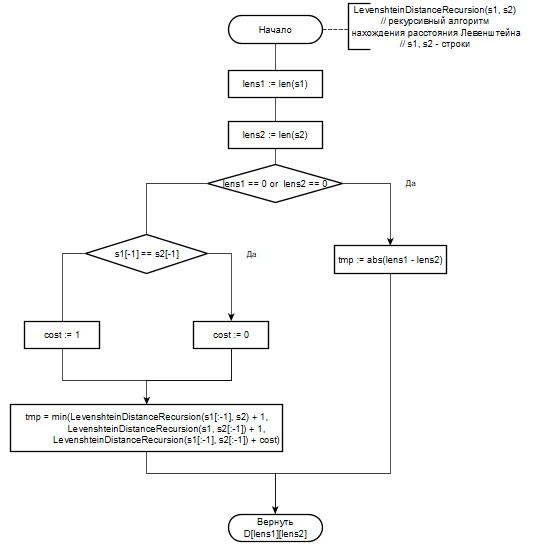
\includegraphics[scale=1]{LevRec}}
	\caption{Рекурсивный алгоритм нахождения расстояния Левенштейна}
	\label{figure:image}
\end{figure}
\newpage
\begin{figure}[h]
	\center{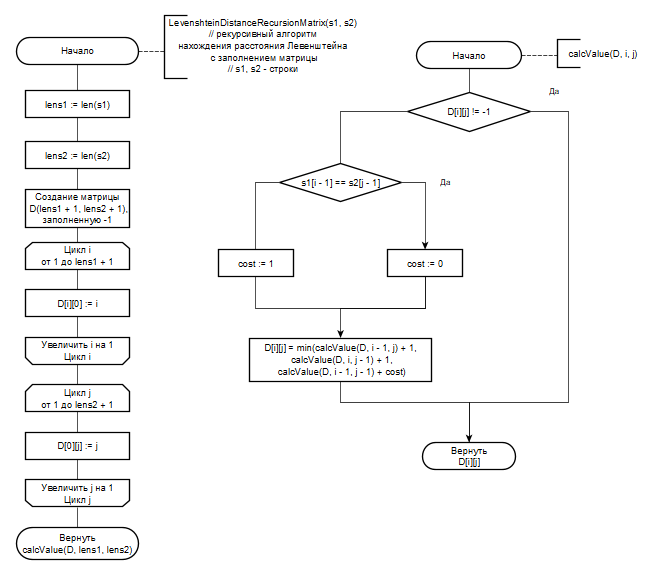
\includegraphics[scale=1]{LevRecMatr}}
	\caption{Рекурсивный алгоритм нахождения расстояния Левенштейна с заполнением матрицы}
	\label{figure:image}
\end{figure}
\newpage
\begin{figure}[h]
	\center{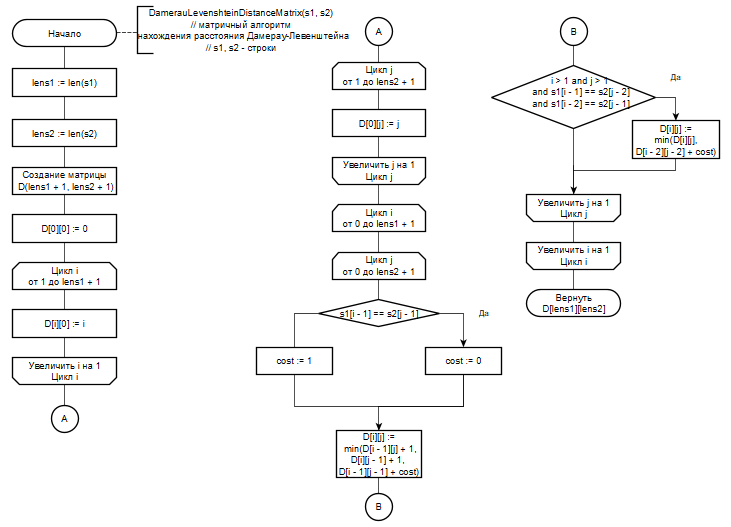
\includegraphics[scale=1]{DamLevMatr}}
	\caption{Рекурсивный алгоритм нахождения расстояния Левенштейна}
	\label{figure:image}
\end{figure}


\chapter{Технологическая часть}
В данном разделе будут рассмотрены требования к программному обеспечению, средства реализации, представлен листинг кода, сравнительный анализ матричной и рекурсивной реализаций, описание тестирования.
\section{Требования к программному обеспечению}
\noindent\textbf{Требования к вводу:}
\begin{enumerate}
	\item на вход подаются две строки;
	\item uppercase и lowercase буквы считаются разными.
\end{enumerate}
\textbf{Требования к программе:}
\begin{enumerate}
	\item две пустые строки — корректный ввод, программа не должна аварийно завершаться;
	\item на выходе
	необходимо получить число, являющиеся результатом работы алгоритма;
	\item для матричных реализаций требуется вывести матрицу решений;
	\item требуется замерить время работы
	каждого из алгоритмов. 
\end{enumerate}
\section{Средства реализации}
В качестве языка программирования был выбран Python т.к. я знаком с данным языком, он простой и лаконичный, имеющий немногословный и понятный синтаксис, похожий на псевдокод, обладающий сильной динамической типизацией, которая способствует быстрому написанию кода. 

Среда разработки — PyCharm, которая предоставляет умную проверку кода, быстрое выявление ошибок и оперативное исправление, вкупе с автоматическим рефакторингом кода, и богатыми возможностями в навигации.  

Матрица создается с помощью функции eye(m, n) из библиотеки numpy \cite{numpy}. 

Время  работы алгоритмов было замерено с помощью функции process\_time() из библиотеки time \cite{time}.

\newpage
\section{Листинг кода}

В листингах 3.1-3.4 представлена реализация алгоритмов нахождения расстояний Левенштейна и Дамерау-Левенштейна

\begin{lstlisting}[label=some-code,caption=Матричный алгоритм нахождения расстояния Левенштейна]
def LevenshteinDistanceMatrix(s1, s2, printMatrix = False):
	lens1 = len(s1)
	lens2 = len(s2)
	D = np.eye(lens1 + 1, lens2 + 1)
	D[0][0] = 0
	for i in range(1, lens1 + 1):
	D[i][0] = i
	for j in range(1, lens2 + 1):
	D[0][j] = j
	for i in range(1, lens1 + 1):
		for j in range(1, lens2 + 1):
			cost = 0 if s1[i - 1] == s2[j - 1] else 1
			D[i][j] = min(D[i - 1][j] + 1, 
								D[i][j - 1] + 1, D[i - 1][j - 1] + cost)

	if printMatrix:
		print('Matrix:')
		outputMatrix(s1, s2, D)
		operations(s1, s2, D)

	return D[lens1][lens2]
\end{lstlisting}

\begin{lstlisting}[label=some-code,caption=Рекурсивный алгоритм нахождения расстояния Левенштейна]
def LevenshteinDistanceRecursion(s1, s2):
	lens1 = len(s1)
	lens2 = len(s2)
	if lens1 == 0 or lens2 == 0:
		tmp = abs(lens1 - lens2)
	else:
		cost = 0 if s1[-1] == s2[-1] else 1
		tmp = min(LevenshteinDistanceRecursion(s1[:-1], s2) + 1,
		LevenshteinDistanceRecursion(s1, s2[:-1]) + 1,
		LevenshteinDistanceRecursion(s1[:-1], s2[:-1]) + cost)
	return tmp
\end{lstlisting}

\newpage
\begin{lstlisting}[label=some-code,caption=Рекурсивный алгоритм нахождения расстояния Левенштейна с заполнением матрицы]
def LevenshteinDistanceRecursionMatrix(s1, s2):
	def calcValue(D, i, j):
		if D[i][j] != -1:
			return D[i][j]
		else:
			cost = 0 if s1[i - 1] == s2[j - 1] else 1
			D[i][j] = min(calcValue(D, i - 1, j) + 1,
			calcValue(D, i, j - 1) + 1,
			calcValue(D, i - 1, j - 1) + cost)
			return D[i][j]

	lens1 = len(s1)
	lens2 = len(s2)
	D = np.full((lens1 + 1, lens2 + 1), -1)
	for i in range(lens1 + 1):
		D[i][0] = i
	for j in range(lens2 + 1):
		D[0][j] = j

	return calcValue(D, lens1, lens2)
\end{lstlisting}

\begin{lstlisting}[label=some-code,caption=Матричный алгоритм нахождения расстояния Дамерау-Левенштейна]
def DamerauLevenshteinDistanceMatrix(s1, s2, printMatrix = False):
	lens1 = len(s1)
	lens2 = len(s2)
	D = np.eye(lens1 + 1, lens2 + 1)
	D[0][0] = 0
	for i in range(1, lens1 + 1):
		D[i][0] = i
	for j in range(1, lens2 + 1):
		D[0][j] = j
	for i in range(1, lens1 + 1):
		for j in range(1, lens2 + 1):
		cost = 0 if s1[i - 1] == s2[j - 1] else 1
		D[i][j] = min(D[i - 1][j] + 1, 
							D[i][j - 1] + 1, D[i - 1][j - 1] + cost)
		if i > 1 and j > 1 and s1[i - 1] == s2[j - 2] and
		 s1[i - 2] == s2[j - 1]:
			D[i][j] = min(D[i][j], D[i - 2][j - 2] + cost)
	
	if printMatrix:
		print('Matrix:')
		outputMatrix(s1, s2, D)
		operations(s1, s2, D)
	return D[lens1][lens2]
\end{lstlisting}

\section{Сравнительный анализ матричной и рекурсивной реализаций}
Рекурсивная реализация работает медленнее по сравнению с матричной из-за повторных вычислений, возникающих в ходе работы рекурсивного алгоритма. Это наглядно видно на Рис. 3.1, иллюстрирующем дерево рекурсивных вызовов. При каждом рекурсивном вызове необходимо передавать в функцию подстроки исходных строк, что затратно по памяти. Эту проблему возможно избежать, если занести строки в глобальные переменные, что является плохой практикой. 

\begin{figure}[ht!]
	\center{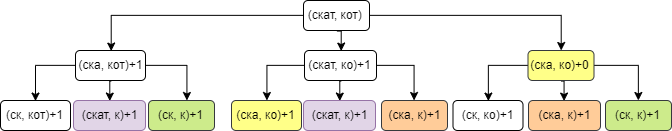
\includegraphics[scale=0.7]{rec.png}}
	\caption{Дерево рекурсивных вызовов}
\end{figure}

Для сравнения, вызов функции, которая реализует матричный алгоритм, происходит один раз и в функцию только один раз передаются обе строки. В этом алгоритме память будет затрачена на хранение матрицы, а время на вложенные циклы, однако затраты будут существенно меньше, чем при многократных вызовах рекурсивной функции.

Пусть длина строки S1 - n, длина строки S2 - m, тогда затраты памяти на приведенные выше алгоритмы будут следующими.
Затраты памяти матричного алгоритма нахождения расстояния Левенштейна:\begin{itemize}
	\item строки S1, S2 - (m + n) * sizeof(char)
	\item матрица - ((m + 1) * (n + 1)) * sizeof(int)
	\item длины строк - 2 * sizeof(int)
	\item вспомогательная переменная - sizeof(int)
\end{itemize}
Затраты памяти рекурсивного алгоритма нахождения расстояния Левенштейна(для каждого вызова):\begin{itemize}
	\item строки S1, S2 - (m + n) * sizeof(char)
	\item длины строк - 2 * sizeof(int)
	\item вспомогательные переменные -  2 * sizeof(int)
	\item адрес возврата
\end{itemize}
 
 Чтобы получить итоговую оценку затрачиваемой памяти необходимо затрачиваемую память для одного вызова умножить на максимальную глубину рекурсии, которая равна сложению длин входных строк.\vspace{\baselineskip}
 
 
 Рекурсивный алгоритм нахождения расстояния Левенштейна с заполнением матрицы:
 \begin{itemize}
	\item матрица - ((m + 1) * (n + 1)) * sizeof(int) 
	\item строки S1, S2 - (m + n) * sizeof(char)
\end{itemize}
 
 Для каждого рекурсивного вызова:
\begin{itemize}
	\item передача данных - 2 * sizeof(int*) + sizeof(int**)
	\item вспомогательная переменная -  sizeof(int)
	\item адрес возврата
\end{itemize}
 
 Чтобы получить итоговую оценку затрачиваемой памяти на рекурсивные вызовы необходимо затрачиваемую память для одного рекурсивного вызова умножить на максимальную глубину рекурсии, которая равна сложению длин входных строк.\vspace{\baselineskip}

Затраты памяти матричного алгоритма нахождения расстояния Дамерау-Левенштейна:\begin{itemize}
	\item строки S1, S2 - (m + n) * sizeof(char)
	\item матрица - ((m + 1) * (n + 1)) * sizeof(int)
	\item длины строк - 2 * sizeof(int)
	\item вспомогательная переменная  - sizeof(int)
\end{itemize}

\section{Описание тестирования}
Реализовано модульное тестирование отдельным файлом test.py с помощью библиотеки unittest \cite{unittest}. Полученные результаты функций сравниваются с контрольными значениями. \vspace{\baselineskip}

Тестирование происходит по следующим данным:
\begin{enumerate}
	\item проверка работы с пустыми строками;
	\item проверка работы с идентичными строками;
	\item проверка работы со строками, имеющие совпадающие символы;
	\item проверка работы с полностью несовпадающими строками.
\end{enumerate}

\chapter{Экспериментальная часть}

В данном разделе приведены примеры работы программы и сравнительный анализ алгоритмов на основе экспериментальных данных. 

\section{Примеры работы} 
 
На рис. 4.1 представлено главное меню программы. 

\begin{figure}[h]
	\center{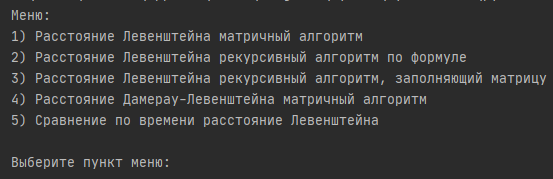
\includegraphics[scale=1]{menu}}
	\caption{Главное меню программы}
	\label{figure:image}
\end{figure} 

На рис. 4.2-4.5 приведены примеры работы программы при вводе строк «тело» и «столб» при выборе пунктов меню 1-4.

\begin{figure}[h]
	\center{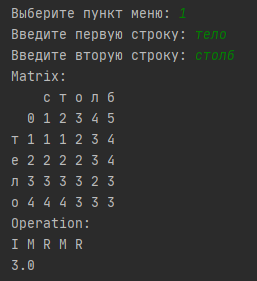
\includegraphics[scale=1]{LevMatrRes}}
	\caption{Результат работы матричного алгоритма нахождения расстояния Левенштейна}
	\label{figure:image}
\end{figure} 

\begin{figure}[h]
	\center{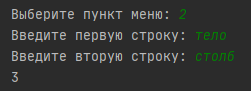
\includegraphics[scale=1]{LevRecRes}}
	\caption{Результат работы рекурсивного алгоритма нахождения расстояния Левенштейна}
	\label{figure:image}
\end{figure} 

\newpage
\begin{figure}[h]
	\center{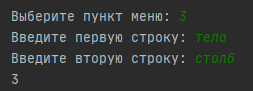
\includegraphics[scale=1]{LevRecMatrRes}}
	\caption{Результат работы рекурсивного алгоритма нахождения расстояния Левенштейна c заполнением матрицы}
	\label{figure:image}
\end{figure} 

\begin{figure}[h]
	\center{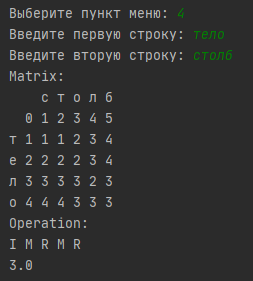
\includegraphics[scale=1]{DauLevMatrRes}}
	\caption{Результат работы матричного алгоритма нахождения расстояния Дамерау-Левенштейна}
	\label{figure:image}
\end{figure} 
\newpage
\section{Результаты тестирования} 
Было проведено тестирование программы, результаты которого занесены в Таблицу 4.1, 1 столбец которой - номер тестового случая; 2 и 3 столбцы - строки, поступающие на вход; 4 и 5 столбец - ожидаемый и полученный результат, в которых приняты следующие обозначения: 
\begin{itemize}
	\item 1-ая цифра – результат работы матричного алгоритма нахождения расстояния Левенштейна
	\item 2-ая цифра – результат работы рекурсивного алгоритма нахождения расстояния Левенштейна
	\item 3-ая цифра – результат работы рекурсивного алгоритма нахождения расстояния Левенштейна с заполнением матрицы;
	\item 4-ая цифра – результат работы матричного алгоритма нахождения расстояния Дамерау-Левенштейна.
\end{itemize}

\newpage
 \begin{table}
	\begin{center}
	\caption{Результаты тестирования}
	\begin{tabular}{| c | c | c | c | c |}
			\hline
			№ & S1 & S2 & Ожидаемый результат & Полученный результат \\
			\hline
			1 & пустая строка & пустая строка & 0, 0, 0, 0 & 0, 0, 0, 0\\
			\hline
			2 & кот & пустая строка & 3, 3, 3, 3 & 3, 3, 3, 3\\
			\hline
			3 & пустая строка & кот & 3, 3, 3, 3 & 3, 3, 3, 3\\
			\hline
			4 & кот & кот & 0, 0, 0, 0 & 0, 0, 0, 0\\
			\hline
			5 & кот & кит & 1, 1, 1, 1 & 1, 1, 1, 1\\
			\hline
			6 & от & кот & 1, 1, 1, 1 & 1, 1, 1, 1\\
			\hline
			7 & кот & кота & 1, 1, 1, 1 & 1, 1, 1, 1\\
			\hline
			8 & кот & кто & 2, 2, 2, 1 & 2, 2, 2, 1\\
			\hline
			9 & кот & рабы & 4, 4, 4, 4 & 4, 4, 4, 4\\
			\hline
	\end{tabular} 
\end{center} 
 \end{table}
 \vspace{\baselineskip}
 Программа успешно прошла все тестовые случаи, все полученные результаты совпали с ожидаемыми. 
\newpage
\section{Постановка эксперимента по замеру времени}

Для произведения замеров времени выполнения реализации алгоритмов будет использована формула: \begin{equation}\label{eq:fourierrow}
	t = \frac{T}{N}
\end{equation}
где t — среднее время выполнения алгоритма, N — количество замеров, T — время выполнения N замеров.  
Неоднократное измерение времени необходимо для получения более точного результа.  
 
 Количество замеров взято равным 100. Эксперимент проводятся на рандомных строках одинаковой длины.


\section{Сравнительный анализ на материале экспериментальных данных}
Для сравнения скорости работы необходимо провести замеры процессорного времени  для строк одинаковой длины.

Был проведены замеры времени работы каждого из алгоритмов, результаты которых занесены в Таблицу 4.2, столбцы которой обозначают следующее: 
\begin{itemize}
	\item 1 столбец – длина строк;
	\item 2 столбец – время работы матричного алгоритма нахождения расстояния Левенштейна;
	\item 3 столбец – время работы рекурсивного алгоритма нахождения расстояния Левенштейна;
	\item 4 столбец – время работы рекурсивного алгоритма нахождения расстояния Левенштейна с заполнением матрицы;
	\item 5 столбец – время работы матричного алгоритма нахождения расстояния Дамерау-Левенштейна.
\end{itemize}
 \newpage
 \begin{table}
	\begin{center}
	\caption{Сравнение алгоритмов по времени(в секундах)}
	\begin{tabular}{|c c c c c|} 
		\hline
		len & LevMatr & LevRec & LevRecMatr & DamLevMatr \\ [0.5ex] 
		\hline\hline
		3 & 0.00000750 & 0.00003239 & 0.00002969 & 0.00000837\\
		\hline
		5 & 0.00008750 & 0.00123438 & 0.00012969  & 0.00008906\\
		\hline
		6 & 0.00009050 & 0.00155438 & 0.00014069  & 0.00009596\\
		\hline
		8 & 0.00024553 & 2.00000438 & 0.00035378  & 0.00026596\\
		\hline
		10 & 0.00029531 & 5.73437500 & 0.00046875 & 0.00032188\\
		\hline
	\end{tabular}
\end{center}
\end{table}

\newpage
 Вывод: У матричных алгоритмов нахождения расстояния Левенштейна время работы пропорционально квадрату длины строк (при увеличении строки в два раза, время увеличивается в четыре раза). Рекурсивный алгоритм по нахождению расстояние Левенштейна показывает наихудшее время, что связано с повторным вычислением одних и тех же значений (пример рис 2.5). Матричный алгоритм по нахождению расстояния Левенштейна и Дамерау-Левенштейна показывают практически одинаковое значение, однако необходимо учитывать то, что Дамерау-Левенштейн решает другую задачу.  

\chapter*{Заключение}
\addcontentsline{toc}{chapter}{Заключение}

В ходе работы были изучены алгоритмы нахождения расстояний Левенштейна и Дамерау–Левенштейна. Реализованы 4 алгоритма поиска этих расстояний, приведен программный код реализации алгоритмов нахождения расстояний.

Было выполнено сравнение разных алгоритмов нахождения расстояния Левенштейна по затраченным ресурсам. Было установлено, что рекурсивный алгоритм занимает гораздо меньше памяти при работе со строками большой длины, чем матричные алгоритмы. Однако матричные алгоритмы отмечаются своим быстродействием.

Цель работы достигнута. Алгоритмы нахождения расстояния Левенштейна и Дамерау-Левенштейна применить на практике, получены практические навыки реализации этих алгоритмов.


\begin{thebibliography}{2}
	\addcontentsline{toc}{chapter}{Список литературы}
	\bibitem{levbook} Дж. Макконнелл. Анализ алгоритмов. Активный обучающий подход. –	М.: Техносфера, 2017. – 267 c. 
	\bibitem{numpy} Библиотека numpy Python, документация [электронный ресурс] – Режим доступа: https://pythonworld.ru/numpy.html, свободный – (Дата обращения: 16.09.20)
	\bibitem{time} Официальный сайт Python, документация [электронный ресурс]. Режим доступа: https://docs.python.org/3/library/time.html, свободный (Дата обращения: 16.09.20)
	\bibitem{unittest} Официальный сайт Python, документация [электронный ресурс] – Режим доступа: https://docs.python.org/3/library/unittest.html, свободный – (Дата обращения: 16.09.20)
\end{thebibliography}
\end{document}